\chapter{Evaluation}

\section{Experimentation with Local Networks}

During software development it is important to be able to adequately test and deploy your software internally on a local network. Although \textit{Mock Routing} is possible, it is only possible to gain a true perspective on how your application functions when it is ran against a real SAFE Network. A network that is both stable and functioning as the global and public SAFE Network would.

\subsection{Method}

After SAFE Wiki was fully working some un-formal experimentation on how well a local SAFE Network can handle the uploading of ZIM files was performed. To do this, a number of \textit{vaults} were setup on different computers on a local network. The computers used included a desktop, laptop and a Raspberry Pi\footnote{https://www.raspberrypi.org/}.

It was very easy to setup the local network, \textit{vaults} could successfully connect to each other and form \textit{sections} without any further configuration. The network was indeed working \textit{autonomously}. Regrettably however, the Raspberry Pi did not work well and consequently it was no longer used. It is difficult to say whether this was down to network connectivity or limited hardware resources. What can be deduced however is that a \textit{vault} running on a machine like a Raspberry Pi 3 is not viable at this time.

ZIM files were repeatedly stored on the network and then browsed from different computers, including computers that didn't have the \textit{vault} running on them. The number of \textit{vaults} on the network was increased to the point that network \textit{splits} started to happen. During testing, the number of \textit{vaults} needed before a \textit{split} happened varied, it did however have a lower bound on the number of \textit{vaults} required. The SAFE Network has a \texttt{split\_buffer} that is used in helping to decide if a network split should happen, currently set to \texttt{3}. This in combination with the \texttt{min\_section\_size} is used to decide if a \textit{split} should happen, the equation can be seen in Figure \ref{fig:split-equation}. For a \textit{split} to happen, this condition must be met for every \textit{section}.

\begin{equation}
	number\ of\ vaults = min\_section\_size + split\_buffer
	\label{fig:split-equation}
\end{equation}

The \texttt{min\_section\_size} is a configuration option that dictates the minimum number of \textit{vaults} required to form a complete \textit{section}. By default this value is set to \texttt{8}, however using this number with a local network is problematic. Using the equation in Figure \ref{fig:split-equation}, to have two \textit{sections} on a local network you would need a minimum of \texttt{22} \textit{vaults}. To run this number of \textit{vaults} on one machine is difficult, anecdotally the network is extremely slow if you do. Hence to facilitate a greater number of \textit{sections} in a local network it is advisable to set the \texttt{min\_section\_size} as small as possible.

\subsection{Results}

What was notable about this experimentation is that it is extremely easy to create your own SAFE Network locally. For developers and researches this facility is of the utmost importance. What proved to be difficult though was varying the \texttt{min\_section\_size} used for the network. It was found that when using a number such as \texttt{2}, the network was unstable. If \textit{vaults} left or joined after data had begun to be stored, the network would cease to function and would simply lock-up and not respond to clients. The explanation for this is that the network isn't designed to be fully functional with such a small \texttt{min\_section\_size}. This means that in practice it is difficult for a single person to have enough computing power to run a local network with a significant number of sections. To have two \textit{sections} with a \texttt{min\_section\_size} of \texttt{2} requires a minimum of \texttt{10} \textit{vaults}. Figure \ref{fig:min-section-size-graph} shows the significance of the difference between a \texttt{min\_section\_size} of \texttt{2} and \texttt{8}.

\begin{figure}
\centering
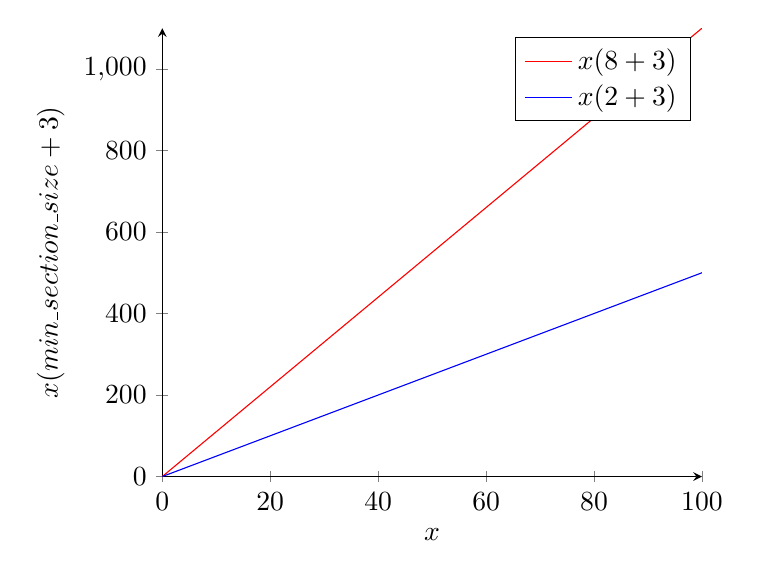
\begin{tikzpicture}
\begin{axis}[
    axis lines = left,
    xlabel = $x$,
    ylabel = {$x(min\_section\_size+3)$},
]
%Below the red parabola is defined
\addplot [
    domain=0:100, 
    samples=100, 
    color=red,
]
{x*(8+3)};
\addlegendentry{$x(8+3)$}
%Here the blue parabloa is defined
\addplot [
    domain=0:100, 
    samples=100, 
    color=blue,
]
{x*(2+3)};
\addlegendentry{$x(2+3)$}
\end{axis}
\end{tikzpicture}

\caption{Compares how \texttt{min\_section\_size} impacts the number of \textit{vaults} needed to form a given number of \textit{sections}.}
\label{fig:min-section-size-graph}
\end{figure}

What this means is that to adequately test an application against a stable and local SAFE Network is difficult. The ability of the network to be more stable at lower \texttt{min\_section\_size} values, or to have a formally specified and endorsed minimum value that can be used, would be very beneficial.

\section{Discussion}

\subsection{Ownership of Data}

As discussed in Section \ref{sec:ownership-of-data}, Ownership of Data is an important aspect of the SAFE Network. ``Users own their own data'' is a feature that the network strives to insure. It is through exploiting these features that developers can create applications in a totally different way.

What needs to be kept in mind however is the Immutability of Immutable Data. Once someone has access to a \textit{Data Map}, the data is available to them indefinitely. There are no permissions to the data that can be tweaked. This means that once a key or access to a \textit{Data Map} is leaked or discovered, that data is available publicly forever. This interacts in odd ways with data de-duplication. Imagine a scenario where a film studio stores an archive of their movies on the SAFE Network. Each film would have its own encrypted \textit{Data Map} that only the studio has the key for. If somehow this file was leaked, a user could upload it to the SAFE Network with an un-encrypted \textit{Data Map}. Owing to \textit{self encryption}, the \textit{Data Map} will then point to the exact same chunks that were stored on the network when the studio originally uploaded that file. Meaning at this point there would be two \textit{Data Maps} that point to the exact same data, an encrypted one and a public one. At this point the studio would have no means of restricting access to the data.

It is thus when using Immutable Data that users have to be extremely careful when managing the keys to that data. Once leaked, there is no method of revoking access. Thankfully most of the key management to such data is handled by storing them inside a users \textit{account} on the network. A chain is as weak as it's weakest link however, leaked \textit{account} credentials means the leak of all of your data with no avenue to reverse the action. Thus the suggestion to further encrypt the data on the client before uploading it to the network, and storing that key through separate means, is highly suggested.

\subsubsection{Immutability of Data}

As mentioned in Section \ref{subsec:immutability-of-data}, data on the SAFE Network is immutable. Once a chunk is written to the network that chunk of data can never be removed. It is the access to data through \textit{Data Maps} and encryption keys that orchestrates the usage of it. What this means in practical situations is that once someone has access to data, they have access to it forever. There is no way to revoke that right. For SAFE Wiki, this is brilliant. Once a ZIM file is uploaded then a user can access that information forever.

What is troubling however is sometimes a user may indeed wish to delete data permanently. To truly have it be gone forever and not stored by the network. This may be on a personal level or asking a company to delete their personal records. Although not implemented yet, there is talk and an RFC\cite{delete-data-rfc} to bring deletable Immutable Data to the network. However to allow ``Immutable Data'' to be deleted is an interesting concept, One can't really call it it ``Immutable'' if you can indeed delete it.

This quality is also why being able to easily run a local test network is crucial. It is not practical to use the ``real'' SAFE Network during testing and development. Not only does this spam the network but also incurs a cost, something that is not acceptable in most scenarios. Thus the importance of being able to easily run a local network that is stable and has multiple \textit{sections} is important.

\subsection{Cost Benefit}
 
A huge benefit to anyone wanting to build a website or application is how much it costs to store data on the SAFE Network. Traditionally on the internet, you would need to pay for a server and also a domain name to be used. Depending on how much traffic the website gets you would need a more powerful server which costs more money. This is not the case on the SAFE Network, the only cost is in writing data. A user could publish a website or blog and it doesn't cost them a penny to keep it on the network, it will be available indefinitely.
 
For SAFE Wiki, this means that once a user pays to upload something like Wikipedia (``only'' ~75GB in size) it is then available to everyone for free and forever. It doesn't cost anymore money than it cost to store the file originally. This means that it is possible to publish a resource like Wikipedia and incur no running costs. As the ZIM file is stored on the network as immutable data it cannot be deleted or altered. Meaning once uploaded that file is available for consumption by all and forever.
 
\subsection{Alternative Business Models}

Like any new technology, the SAFE Network opens up many opportunities that didn't exist before. In SAFE Network nomenclature, \textit{vaults} farm data. The safe and reliable storage (farming) of data is rewarded with \textit{Safecoin}. 

\subsubsection{Exploiting Consumer Resources}

One could envision an application that instead of charging users for access, allows them to become a \textit{vault} that generates \textit{Safecoin}. This \textit{Safecoin} could then be sent back to the creators of the program and hence financially compensates them for the usage of their application. One consideration of this approach however is that \textit{vaults} don't get to choose what data they store, that is an integral part of the architecture of the SAFE Network. By following this financial model then it would be for the ``good of the whole'', increasing the utility of the entire network and not just for one application.

This model could be used to better make use of a consumers resources. When a user sits and watches Netflix on an entertainment system, there is very little strain on the resources of the device. In the case of a games console, literally teraflops of processing power, advanced networking and storage facilities are going unused. Potential financial models can try to \textit{exploit} this untapped power to the benefit of both the user and the provider of the application. Encouraging the creation of more \textit{vaults} not only increases the utility of the SAFE Network but provides users with an entirely new way to pay for content. Offering the resources they have in exchange for access to services.

\subsubsection{Micro-Payments}

As \textit{Safecoin} is so tightly integrated with the network it can be used in interesting ways. A possibility talked about in the \textit{Safecoin} white-paper\cite{lambert2015safecoin} is the facilitation of micro-payments. Traditional currencies and payment processing methods are too expensive to be used for quick and small payments, hence why many merchants will charge a fee to use a card machine. This issue does not exist for \textit{Safecoin} which means it can be used to facilitate small payments. To give an example, a music artist could upload their discography to the SAFE Network and link their wallet to the files via some mechanism. As users listen to the song (read the chunks from the network), \textit{Safecoin} could be sent from their wallet(s) dynamically based upon their consumption of the music. As the white-paper suggests, this could even be used ``to pay for films on a cost per frame basis, with the user only paying for what they watch''. By using this system, artists and creators could cut out the ``middle-man'' for users consuming their content. If the financial benefits are significant then they may be drawn to the SAFE Network over alternative platforms like Spotify. Current platforms usually take a significant cut of profits so it may indeed result in higher revenue for them. How profitable a system like this would be remains to be seen. When Maidsafe gives a formal outline of how micro-payments will be implemented it will then be possible to examine if they will benefit creators.

\subsection{Privacy and Anonymity}

Anonymity and Privacy are not mutually exclusive. Anonymity means \textit{``Nameless; of unknown name; also, of unknown or unavowed authorship''}\cite{anonymous}. True anonymity is very important for many people around the world, especially when it comes to digital communications. The identities of individuals is what matters here. Being able to convey a message and be ``nameless''. 

Privacy means \textit{``The state of being in retirement from the company or observation of others; seclusion''}\cite{privacy}. Privacy is an important aspect of our lives that some hold to a higher virtue than others. Most would agree however that you should be able to send a message/letter/email to someone and have that communication be private.

To relate the two concepts together in terms of the SAFE Network, I would say that anonymity relates to meta-data and privacy relates to data itself. A real world example of meta-data is something like an address. When you send a letter to someone, the postal service can see the address on the envelope. The letter is not anonymous because the recipient is not ``nameless''. The contents of the envelope, the data, is however private between the two parties. It is \textit{``in retirement from the company or observation of others''}. The SAFE Network provides guarantees of privacy. A user could upload pictures and documents with the assurance that only they can access them, it is private data. A user could also send a message to someone by inserting an encrypted entry in their ``inbox'', again this allows private communication. When a client requests a chunk of data from a vault, that vault knows something relating to the \textit{account} that is requesting the data. However difficult it may be to tie that information to an individual, that information exists for a period of time and hence full anonymity is not insured.

This has big implications for the use case of the network but the nuances of how this impacts things is quite subtle. \textit{Data Maps} are what gives meaning and relationship to chunks of data. At the storage level, chunks have absolutely no discernible relationship to each other. The access to \textit{Data Maps} is what gives users privacy. If you are the only person who knows where it is and how to decrypt it then the data it leads to is truly private. Once data is stored on the network, it is anonymous. Thus for the above reasons the SAFE Network allows pseudo-anonymised interactions. In practically users can be relatively assured that their interaction is anonymous, they must however know that it is non ensured fully.

Privacy and anonymity is very important for SAFE Wiki. In some parts of the world people do not have the freedom to access any information they want. A modern day example of this is that the Chinese government are still censoring access to information about Tiananmen Square\cite{tiananmen-square}. Thus the privacy and pseudonymization of activity is very important. The SAFE Network facilitates the uncensored access to information, which as discussed at the beginning of this report is crucial to developing societies. If a user can connect to the SAFE Network successfully they can interact with it fully, there is no avenue to censor or curate their interactions.

\subsection{Building websites on the SAFE Network}

The SAFE Network can do simple websites really well. If a user wants to create a blog or a website then the SAFE Network is a fabulous choice. The cost benefit of not having ``running costs'' is a big benefit to people. Some websites are not updated frequently and thus being stored on the SAFE Network would possibly save users years of running costs. It is when websites become more complex, that the SAFE Network becomes a very difficult product to suggest. A simple example is e-commerce. As there is no processing available on the SAFE Network you would have to run your website against a server to handle payment processing. With that, it almost breaks the point of using the SAFE Network to some degree. It is still useful but by relying on a server makes one wonder if there is much point in using the SAFE Network to host the website. Some shops may find it more profitable but for some there may be little benefit. This could be answered by offering the use of Cryptocurrency as an option to pay for goods, this approach wouldn't need a traditional server to handle payment processing. For wide-scale adoption however only accepting Cryptocurrency is not a sensible option.

\subsection{Storing and archiving data}

The storage of data is where the SAFE Network excels. Immutable Data on the SAFE Network is immutable. Storing things like backups and archives makes perfect sense, once stored it cannot be removed. Thus the SAFE Network is a very attractive option when it comes to the long term and secure storage of data, this applies to organisations and to individual users. The general populous could make very good use of services like DropBox on the SAFE Network. The attractive thing about this is that they can know their data is safe, only they have access to it. The reduced cost is very appealing too, a user could backup large amounts of data and have access to it indefinitely without having to pay a yearly or monthly fee. Organisations could use the SAFE Network to perform backups of critical systems and for other purposes. Long term indefinite storage with a one time fee is a very attractive prospect.

\subsubsection{Companies cannot own third party data}

As discussed previously, data on the SAFE Network cannot be deleted. This means that under current laws and regulations, companies would find it extremely difficult to operate under their current methods. If for instance a user requested that their data was deleted, the company simply wouldn't be able to if it was stored on the SAFE Network. All they could do is the equivalent of throwing away the key to a filing cabinet. Amongst many other reasons, this is why companies cannot own ``third party'' data on the SAFE Network. How this is handled needs to be flipped to a model where users/companies own their own data. Instead of a user giving companies their data, they give the companies access to their data to facilitate the services they wish to access. This model means that services would need to be built around the idea that the source of the data is ultimately in control of that data. For services like Netflix\footnote{https://www.netflix.com/}, this would mean that the content produces would simply grant access to their videos and Netflix would then simply exist as an intermediary between the consumer and the video. This model means the content producer owns their own content.

\section{Future Improvements to SAFE Wiki}

Future work for SAFE Wiki could take one of two approaches. Development could continue on SAFE Wiki itself or another approach could be taken, using the lessons learned from developing SAFE Wiki. An alternative approach to how SAFE Wiki could develop is outlined below.

\subsection{ZIM Uploader}

The first step would be to create a new application called ``ZIM Uploader''. This applications only purpose would be to facilitate the management of ZIM files on the SAFE Network. This means that the average user that has no intention of uploading their own ZIM file doesn't need to see this piece of functionality. As this application only serves one purpose it would be far easier to maintain than SAFE Wiki itself.

Indeed it is highly likely that other developers will create applications to facilitate NFS usage on the SAFE Network. As long as they allow users to create a ZIM Folder and place files within them using NFS emulation, then they could be used to manage ZIM files on the network. Remember there really isn't anything special about a ZIM Folder, it is just a MD structure that is emulated through NFS to store ZIM files. If this happens then the maintenance of a ``ZIM Uploader'' would no longer be required.

\subsection{Kiwix JS Extension}
\label{subsec:kiwix-js-safe}

Kiwix JS itself is a browser extension, using the browser as its run-time environment. Forking away from this approach perhaps fragments things more than they need to be. Instead of pulling Kiwix JS into a desktop application, through the use of the \textit{Web API} the functionality of SAFE Wiki could be brought to the extension. With this approach the user would have Kiwix JS installed inside their browser (SAFE Browser or Peruse) and be able to use Kiwix JS as normal. Within a SAFE Network environment, Kiwix JS would then have the ability to read ZIM files from the SAFE Network.

Extending Kiwix JS functionality instead of forking it brings many benefits. The first and foremost is that there is the possibility of this added functionality being merged into the main branch of Kiwix JS. Meaning it would be a supported solution provided by Kiwix. This would not only increase the awareness of ``SAFE Wiki'' but means that improvements (bug fixes etc) can be made to one single repository instead of constantly pulling changes across the two streams. As it would only have the functionality to read ZIM files, the changes required are minimal when compared to all the changes that happened inside SAFE Wiki. This approach makes sense, SAFE Wiki simply facilitates another storage medium for Kiwix JS to use.

\subsection{Website}

Through the \textit{Web API} it would be possible to build a website that would facilitate the reading of ZIM files. This means a user could simply visit the website through a SAFE Network compatible browser and then browse ZIM files hosted on the network as they wish. This approach would deliver the internals of Kiwix JS through the browser to run on the client, providing users with an extremely easy method to access the functionality of SAFE Wiki. This approach however does have its drawbacks. It would mean the maintenance of another code base meaning the benefits described in Section \ref{subsec:kiwix-js-safe} would not apply.

\subsection{Suggestion}

The big downside with choosing to build a website would be that users lose the ability to view ZIM files that they have stored locally. One can envision that in the future it would be possible for a user to download ZIM files from the SAFE Network for offline consumption. Thus maintaining the ability to browse the files locally, without an internet connection, is a key piece of functionality that shouldn't be lost. Thus the preferred and suggested approach is the one outlined in Section \ref{subsec:kiwix-js-safe}. It is Kiwix JS, a well established project, with the added ability to read files from the SAFE Network.

\section{Unresolved Questions and Problems with the SAFE Network}

\subsection{Performance}
\label{subsec:problem-performance}

How practical the SAFE Network will be for applications like video streaming and file downloads is unknown at this point. Speaking from experience, dealing with uploading large quantities of data to a local SAFE Network is slower than one might imagine. Although this observation is merely anecdotal it will be interesting to see what performance is like when there is a global SAFE Network. How \textit{node ageing} and \textit{churn} effect performance is also an interesting question to ponder. When \textit{vaults} are moving between \textit{sections}, those \textit{vaults} no longer contribute to the resources of a particular \textit{section} and actually consume them instead. Thus how these network events impact on the experience of the end-user is still to be seen.

\subsection{Safecoin}
\label{subsec:problem-safecoin}

The fee model and economy of \textit{Safecoin} is not well established. The \textit{Safecoin} white-paper\cite{lambert2015safecoin} does give some indications as to how things will work but the implementation details are omitted. The economy of \textit{Safecoin} is crucial for the success of the SAFE Network, if it doesn't work then the network itself will not function. The disbursement of coins through \textit{farming} and other means is an interesting question that needs to be answered. There have been talks about rewarding developers for usage of their application and also rewarding creators for reads of their content. Imagine a Spotify where users directly pay artists when they listen to the content, no middle man needed. Another critical point that is worrisome is how \textit{farming} rewards the \textit{vault} owners. In the white-paper on \textit{Safecoin} it is said that \textit{Safecoin} is awarded ``to the successful node as data is retrieved from it (GETS), as opposed to when it is stored (PUTS)''. This does make sense to some degree but in others leaves a lot unanswered. What this means is that if data is never accessed, the \textit{vaults} storing that data will never be rewarded for doing so. This means that the network has to support the data indefinitely and nobody will ever be incentivised for doing so. This means that  the amount of \textit{Safecoin} that was originally used to pay for the storage of the data has to be great enough to cover storage and network costs for decades upon decades. That simply doesn't make sense. A possible answer to this is that \textit{vaults} are paid during \textit{churn} when they send and receive data to one another, this is a mere guess however and is not specified in the white-paper.

\subsection{Maidsafe has an information problem}

The situation regarding documentation makes suggesting working with the SAFE Network extremely difficult. The main problem is the lack of clarity and ``cannon'' knowledge on different subjects. There is no central location where a developer could lookup a piece of information and get the hard facts as to what they are enquiring about. Information is spread thin and far across the forums and different blog websites. Sometimes it is hard to distinguish between opinions on how things should be and how they actually are. Indeed the Wiki for the SAFE Network is incredibly out of date in some areas, some of it is just plain wrong. This issue resulted in some very kind community members taking it upon themselves to write the \citetitle{safe-network-primer} document. This document is one of the first unified resources of information that people can use to learn about the SAFE Network. One of the only that goes into enough detail to explain the network properly. This speaks to the enthusiasm of the community at large who believe in the SAFE Network and its ultimate utility. There is a lot of knowledge out there, it just needs to be brought into one central location that is an approved resource of knowledge.

This lack of clarity can be explained, but not excused, by the infancy of the network. It is only in \textit{alpha 2} and not a finished product. Going forward however this is something that needs to be addressed. It is certainly something that made assembling information for this dissertation very difficult.

\subsection{How Traditional Internet Businesses would Benefit}

Suggesting that the SAFE Network is a viable avenue for existing business is difficult. A few basic details mean that their current financial models simply wouldn't work on the SAFE Network. Basic financial models like subscription based services is difficult to even imagine how they would be implemented on the SAFE Network. Thus how traditional businesses  would benefit from the architecture of the SAFE Network is a very difficult question to answer. Thus the suggestion is that many simply do not benefit. For most, their entire business is based around the collection and curation of user data and thus the SAFE Network is not commercially viable to them. Thus new models on how to commercialise a business idea will have to be thought of. The main barrier to this is the technical challenges in how to do so. The SAFE Network is incredibly rigid when compared to the flexibility of the traditional model of the internet thus there has to be the creative exploration of how to facilitate and incentivise existing services to move across to the SAFE Network.

\subsection{A Full Prototype Doesn't Exist}

To date there isn't a fully working prototype of what the ``1.0'' release of the network will be. At this point, it is crucial that the network works properly as users will see this as the signal to start storing important data. In extension to this, a succinct and official definition of what the SAFE Network will be isn't available. Thus the current version of the SAFE Network is nothing more than a demo, work in progress, for what the ``final'' version of the network will be. This makes it extremely difficult to draw any sort of concrete conclusions as to the effectiveness of the network and developing applications for it.

\subsection{Future Work}

The SAFE Network provides many exciting avenues for academic research. The title of this paper is ``Building Applications on the SAFE Network'' and that was the main focus of it. With such a broad topic it is difficult to answer some specific questions in as much depth that is needed. The following are proposals of specific areas that would benefit from explicit  and deep academic research.

\subsubsection{Safecoin}

As discussed in Section \ref{subsec:problem-safecoin}, the success of \textit{Safecoin} is crucial to the success of the SAFE Network. A deeper and formal analysis on the economic viability of the \textit{Safecoin} is needed to really evaluate whether the SAFE Network is a financially viable option for users.

\subsubsection{Datachain's}

How Datachain's will ultimately impact the operation of the SAFE Network is still undecided. An interesting academic exercise could be to review the current proposals and to run simulations to give quantitative evidence to the effectiveness of those proposals. They are implementing the current proposals and will be included in the \textit{alpha 3} release of the network. Upon the successful release of \textit{alpha 3} the deeper analysis of how Datachain's operate and function will be possible. This is all information that would be incredibly useful to Maidsafe.

\subsubsection{Competitors}

There does exist some competitors to the SAFE Network and they all share the central goal of creating a decentralised peer to peer file storage network. An analysis on how the SAFE Network compares to these competitors would be an interesting topic to look at. An ideal candidate for comparison is Filecoin\cite{filecoin}. The goals of both projects is very similar but with different ways to achieve the same goals. The incentive layer for Filecoin is far more clearly defined than in the SAFE Network (currently) so an evaluation between the two could be beneficial academically and to Maidsafe themselves.




